\documentclass[]{article}
\usepackage[utf8]{inputenc}
\usepackage[ngerman]{babel}
\usepackage[T1]{fontenc}
\usepackage{%
	ngerman,
	ae,
	times,  %% hier kann man die Schriftart einstellen
	graphicx,
	url,
	scrlayer-scrpage,
	lastpage,
	mathtools,
	geometry,
	multicol,
	cancel,
	xcolor,
	nicematrix,
	xfrac,
	tikz,
	pgfplots,
	amsmath,
	colortbl,
	centernot,
	dsfont,
	textgreek,
	icomma,
	pdfpages}
\usepackage[thinlines]{easybmat}
\usetikzlibrary{datavisualization}
\usetikzlibrary{datavisualization.formats.functions}
\usetikzlibrary{intersections}
\pgfplotsset{compat=1.17}
\newcommand{\del}[1]{\cancel{~#1~}}
\NiceMatrixOptions{ last-col,code-for-last-col = \color{blue}\scriptstyle,light-syntax}
\newlength\dlf
\newcommand\alignedhighlight[3]{
  % #1 = color
  % #2 = before alignment
  % #3 = after alignment
  &
  \begingroup
  \settowidth\dlf{$\displaystyle #2$}
  \addtolength\dlf{\fboxsep+\fboxrule}
  \hspace{-\dlf}
  \fcolorbox{#1}{#1}{$\displaystyle #2 #3$}
  \endgroup
}
\newcommand{\reference}[1]{ \text{\small{\textcolor{blue}{(#1)}}} }

\newcommand{\topic}{Grundlagen Technische Informatik}
\newcommand{\subtopic}{Übung 1}
\newcommand{\authors}{Nils Helming}

%Head and Footnotes
\setlength{\headheight}{2.1\baselineskip} %baselineskip = minimum distance bbetween the bottom of one line to another.
\geometry{bottom = 3cm}
\setlength{\headsep}{\baselineskip}
\ihead[\topic\hrule]{\topic\hrule}
\chead[\subtopic\\~]{\subtopic\\~}
\ohead[\authors\\~]{\authors\\~}
\ifoot[~]{~}
\cfoot[~]{~}
\ofoot[Seite \thepage~von \pageref{LastPage}]{Seite \thepage~von \pageref{LastPage}}

%Paragraph spacings
\setlength{\parindent}{0em} %em = with of an 'M'
\setlength{\parskip}{1ex} %ex = height of an 'x'


\newcommand{\V}{\lor}
\newcommand{\A}{\land}
\newcommand{\T}[1]{\overline{#1}}
\newcommand{\eq}{\Leftrightarrow}
\newcommand{\rarr}{\Rightarrow}
\newcommand{\red}[1]{\textcolor{red}{#1}}

\newcommand{\unit}[1]{\text{#1}}
\newcommand{\fracunit}[2]{\frac{\unit{#1}}{\unit{#2}}}
\newcommand{\textsq}[1]{\ensuremath{\text{#1}^2}}
\newcommand{\textpow}[2]{\ensuremath{\text{#1}^{#2}}}
\newcommand{\tdot}{\ensuremath{\cdot}}


\begin{document}
\section*{Aufgabe 1:}
\subsection*{(a)}
	\begin{align*}
		&& Y &= [(A \A \T{B})\V (\T{C} \A D) \V \T{E} \V F] \A G &&\\
		&& \T{Y} &= [(\T{A} \V B)\A (C \V \T{D}) \A E \A \T{F}] \V \T{G} &&\\
	\end{align*}
\subsection*{(b)}
	\begin{multicols*}{2}
	\begin{align*}
		\text{0000000:}&& Y &= [(0 \A \T{0})\V (\T{0} \A 0) \V \T{0} \V 0] \A 0 &&\\
		&& &= [(0 \A 1)\V (1 \A 0) \V 1 \V 0] \A 0 &&\\
		&& &= [(0)\V (0) \V 1 \V 0] \A 0 &&\\
		&& &= [1] \A 0 &&\\
		&& &= 0 &&\\
		&& \T{Y} &= [(\T{0} \V 0)\A (0 \V \T{0}) \A 0 \A \T{0}] \V \T{0} &&\\
		&& &= [(1 \V 0)\A (0 \V 1) \A 0 \A 1] \V 1 &&\\
		&& &= [(1)\A (1) \A 0 \A 1] \V 1 &&\\
		&& &= [0] \V 1 &&\\
		&& &= 1 &&\\
	\end{align*}

	\begin{align*}
		\text{1111111:}&& Y &= [(1 \A \T{1})\V (\T{1} \A 1) \V \T{1} \V 1] \A 1 &&\\
		&& &= [(1 \A 0)\V (0 \A 1) \V 0 \V 1] \A 1 &&\\
		&& &= [(0)\V (0) \V 0 \V 1] \A 1 &&\\
		&& &= [1] \A 1 &&\\
		&& &= 1 &&\\
		&& \T{Y} &= [(\T{1} \V 1)\A (1 \V \T{1}) \A 1 \A \T{1}] \V \T{1} &&\\
		&& &= [(0 \V 1)\A (1 \V 0) \A 1 \A 0] \V 0 &&\\
		&& &= [(1)\A (1) \A 1 \A 0] \V 0 &&\\
		&& &= [0] \V 0 &&\\
		&& &= 0 &&\\
	\end{align*}

	\begin{align*}
		\text{1010101:}&& Y &= [(1 \A \T{0})\V (\T{1} \A 0) \V \T{1} \V 0] \A 1 &&\\
		&& &= [(1 \A 1)\V (0 \A 0) \V 0 \V 0] \A 1 &&\\
		&& &= [(1)\V (0) \V 0 \V 0] \A 1 &&\\
		&& &= [1] \A 1 &&\\
		&& &= 1 &&\\
		&& \T{Y} &= [(\T{1} \V 0)\A (1 \V \T{0}) \A 1 \A \T{0}] \V \T{1} &&\\
		&& &= [(0 \V 0)\A (1 \V1) \A 1 \A 1] \V 0 &&\\
		&& &= [(0)\A (1) \A 1 \A 1] \V 0 &&\\
		&& &= [0] \V 0 &&\\
		&& &= 0 &&\\
	\end{align*}

	\begin{align*}
		\text{0101010:}&& Y &= [(0 \A \T{1})\V (\T{0} \A 1) \V \T{0} \V 1] \A 0 &&\\
		&& &= [(0 \A 0)\V (1 \A 1) \V 1 \V 1] \A 0 &&\\
		&& &= [(0)\V (1) \V 1 \V 1] \A 0 &&\\
		&& &= [1] \A 0 &&\\
		&& &= 0 &&\\
		&& \T{Y} &= [(\T{0} \V 1)\A (0 \V \T{1}) \A 0 \A \T{1}] \V \T{0} &&\\
		&& &= [(1 \V 1)\A (0 \V 0) \A 0 \A 0] \V 1 &&\\
		&& &= [(1)\A (0) \A 0 \A 0] \V 1 &&\\
		&& &= [0] \V 1 &&\\
		&& &= 1 &&\\
	\end{align*}
	\end{multicols*}
\section*{Aufgabe 2:}
	\begin{align*}
		&& Y &= (\T{A} \A (\T{B}\V \T{C})) \V (D \A \T{E} \A F) &&\\
	\end{align*}
\subsection*{(a)}
	\begin{align*}
		&& Y &= (\T{A} \A (\T{B}\V \T{C})) \V (D \A \T{E} \A F) &&\\
		&& &= (\T{A} \A \T{(B \A C)}) \V \T{\T{(D \A \T{E} \A F)}} &&\\
		&& &= \T{\T{(\T{A} \A \T{(B \A C)})}} \V \T{\T{(D \A \T{E} \A F)}} &&\\
		&& &= \T{\T{(\T{A} \A \T{(B \A C)})} \A \T{(D \A \T{E} \A F)}} &&\\
		&& &= \T{\T{\T{A} \A \T{B \A C}} \A \T{D \A \T{E} \A F}} &&\\
	\end{align*}
\subsection*{(b)}
	\begin{align*}
		&& Y &= \T{\T{\T{A} \A \T{B \A C}} \A \T{D \A \T{E} \A F}} &&\\
		&& &= \T{\T{(\T{A}) \A (\T{B \A C}}) \A (\T{D \A (\T{\T{\T{E} \A F}})}}) &&\\
	\end{align*}
\subsection*{(c)}
	\begin{center}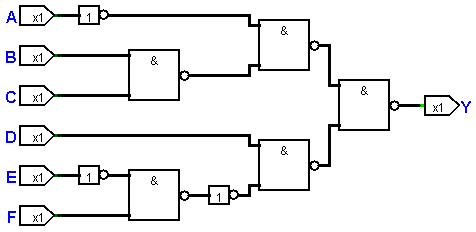
\includegraphics[scale=0.7]{Bilder/2_c.png}\end{center}

\section*{Aufgabe 3:}
	\begin{align*}
		&& Y &= (A \V \T{B}) \A \T{C} &&\\
		&& h(A,B,C) &= (A \V \T{B}) \A \T{C} &&\\
		&&  &= (\T{\T{A}} \V \T{B}) \A \T{C} &&\\
		\\
		&& g(A,B,C) &= \T{h(A,B,C)} &&\\
		\text{nach Shannonsches Gesetz:}&&  &= (\T{A} \A B) \V C &&\\
	\end{align*}
	\begin{center}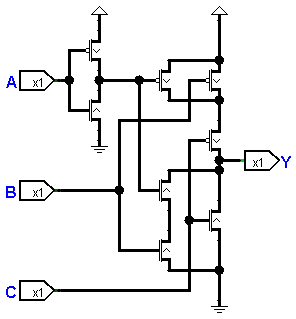
\includegraphics[scale=0.7]{Bilder/3.png}\end{center}

\section*{Aufgabe 4:}
	\begin{align*}
		&& F &= (F1 \V F2 \V F3) \A F4 &&\\
		&& F1&= \T{A} \A B &&\\
		&& F2&= A \A B &&\\
		&& F3&= A \A \T{B} \A \T{C} &&\\
		&& F4&= \T{A} \V C \V A &&\\
		\\
		&& F1 \V F2&= (\T{A} \A B) \V (A \A B) &&\\
		&& &= B &&\\
		\\
		&& F4&= \T{A} \V C \V A &&\\
		&& &= 1 &&\\
		\\
		\rarr&& F &= (F1 \V F2 \V F3) \A F4 &&\\
		&&  &= B \V F3 &&\\
	\end{align*}
	\newcommand{\dbl}[2]{\begin{matrix}#1 \\ #2\end{matrix}}
	\begin{center}$\begin{BMAT}(){c|c|c|c|c|c|c}{c|cccccccc}
		A & B & C & \T{B} 	& \T{C}	&\dbl{F3=}{A \A \T{B} \A \T{C}}	& \dbl{F =}{B \V F3}\\
		0 & 0 & 0 & 1 		& 1		& 0								& 0\\
		0 & 0 & 1 & 1 		& 0		& 0								& 0\\
		0 & 1 & 0 & 0 		& 1		& 0								& 1\\
		0 & 1 & 1 & 0 		& 0		& 0								& 1\\
		1 & 0 & 0 & 1 		& 1		& 1								& 1\\
		1 & 0 & 1 & 1 		& 0		& 0								& 0\\
		1 & 1 & 0 & 0 		& 1		& 0								& 1\\
		1 & 1 & 1 & 0 		& 0		& 0								& 1\\
	\end{BMAT}$\end{center}
\newpage
\section*{Aufgabe 5:}
\begin{center}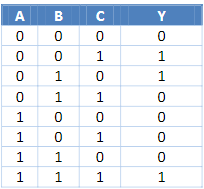
\includegraphics[scale=0.7]{Bilder/5.png}\end{center}
\subsection*{(a)}
	folgende Minterme sind hier relevant:
	\begin{align*}
		&& m_1 &= \T{A} \A \T{B} \A C &&\\
		&& m_2 &= \T{A} \A B \A \T{C} &&\\
		&& m_7 &= A \A B \A C &&\\
	\end{align*}
\subsection*{(b)}
	Die DNF ist dann die Disjunktion der Minterme:
	\begin{align*}
		&& Y &= m_1 \V m_2 \V m_7 &&\\
		&& &= (\T{A} \A \T{B} \A C) \V (\T{A} \A B \A \T{C}) \V (A \A B \A C) &&\\
	\end{align*}
\subsection*{(c)}
	folgende Maxterme sind hier relevant:
	\begin{align*}
		&& M_0 &= \T{A} \A \T{B} \A \T{C} &&\\
		&& M_3 &= \T{A} \A B \A C &&\\
		&& M_4 &= A \A  \T{B} \A \T{C} &&\\
		&& M_5 &= A \A \T{B} \A C &&\\
		&& M_6 &= A \A B \A \T{C} &&\\
	\end{align*}
	Die KNF ist dann die Konjunktion der Maxterme:
	\begin{align*}
		&& Y &= M_0 \A M_3 \A M_4 \A M_5 \A M_6 &&\\
		&& &= (\T{A} \A \T{B} \A \T{C}) \A (\T{A} \A B \A C) \A (A \A  \T{B} \A \T{C}) \A (A \A \T{B} \A C) \A (A \A B \A \T{C}) &&\\
	\end{align*}
\subsection*{(d)}
	\begin{center}$\begin{BMAT}(){c|c|c|c|c|c|c}{c|cccccccc}
		A & B & C & Y & m_1	& m_2	& m_7\\
		0 & 0 & 0 & 0 & 0	& 0		& 0\\
		0 & 0 & 1 & 1 & 1	& 0		& 0\\
		0 & 1 & 0 & 1 & 0	& 1		& 0\\
		0 & 1 & 1 & 0 & 0	& 0		& 0\\
		1 & 0 & 0 & 0 & 0	& 0		& 0\\
		1 & 0 & 1 & 0 & 0	& 0		& 0\\
		1 & 1 & 0 & 0 & 0	& 0		& 0\\
		1 & 1 & 1 & 1 & 0	& 0		& 1\\
	\end{BMAT}$\end{center}

\subsection*{(e)}
	\begin{center}$\begin{BMAT}(){c|c|c|c|c|c|c|c|c}{c|cccccccc}
		A & B & C & Y & M_0	& M_3	& M_4	& M_5	& M_6\\
		0 & 0 & 0 & 0 & 0	& 1		& 1		& 1		& 1\\
		0 & 0 & 1 & 1 & 1	& 1		& 1		& 1		& 1\\
		0 & 1 & 0 & 1 & 1	& 1		& 1		& 1		& 1\\
		0 & 1 & 1 & 0 & 1	& 0		& 1		& 1		& 1\\
		1 & 0 & 0 & 0 & 1	& 1		& 0		& 1		& 1\\
		1 & 0 & 1 & 0 & 1	& 1		& 1		& 0		& 1\\
		1 & 1 & 0 & 0 & 1	& 1		& 1		& 1		& 0\\
		1 & 1 & 1 & 1 & 1	& 1		& 1		& 1		& 1\\
	\end{BMAT}$\end{center}




\end{document}